\documentclass{book}
\usepackage{fontspec}
\usepackage{alltt}
\usepackage{xcolor}
\usepackage{pdfpages}
\setmainfont{NotoSerif}
\newfontfamily\fcmd{NotoSans}[Colour=blue,NFSSFamily=noto,Scale=4]
\newcommand\cmd[1]{{\fcmd#1}}
\newcommand\ffontname{Yinit}
\newfontfamily\fsample{\ffontname}[Colour=red,Scale=4]

\newcommand\xletttextdiv{\ \par
\noindent
:\hfill\rule{0.32\textwidth}{0.5pt}\hfill :
\par}

\newcommand\xlettrinehelptext{%
x x x x x x x x x x x x x x x x x x x x  xx x x x x x x 
x x x x x x x x x x x x x x x x x x x x  xx x x x x x x 
x x x x x x x x x x x x x x x x x x x x  xx x x x x x x 
x x x x x x x x x x x x x x x x x x x x  xx x x x x x x 
x x x x x x x x x x x x x x x x x x x x  xx x x x x x x 
x x x x x x x x x x x x x x x x x x x x  xx x x x x x x 
x x x x x x x x x x x x x x x x x x x x  xx x x x x x x 
x x x x x x x x x x x x x x x x x x x x  xx x x x x x x 
x x x x x x x x x x x x x x x x x x x x  xx x x x x x x 
x x x x x x x x x x x x x x x x x x x x  xx x x x x x x 
}

\newcommand\xchapter[1]{\xletttextdiv\chapter{#1}\xlettrine}



	
\ExplSyntaxOn


\bool_new:N \l_xlett_legacyfont_bool % true for legacy fonts
\fp_new:N \l_xlett_vfactor_fp % how much of lettrine to move para up by, e.g., -1.3 times
\tl_new:N \l_xlett_font_tl % for legacy fonts, e.g., \input Acorn.fd
\dim_new:N \l_xlett_font_size_dim % for legacy fonts, e.g., 60pt
\dim_new:N \l_xlett_font_baselineskip_dim % for legacy fonts, e.g., 72pt
\tl_new:N \l_xlett_font_type_tl % for legacy fonts, e.g., T1
\tl_new:N \l_xlett_font_family_tl % for legacy fonts, e.g., Acorn
\tl_new:N \l_xlett_font_series_tl % for legacy fonts, e.g., m
\tl_new:N \l_xlett_font_shape_tl % for legacy fonts, e.g., n
\tl_new:N \l_xlett_firstword_tl
\tl_new:N \l_xlett_initial_tl

\dim_new:N \l_xlett_initkern_dim % of first word's tail, e.g., -0.3em
\dim_new:N \l_xlett_indentbuffer_dim % space around lettrine, e.g., 0.4em





\keys_define:nn { xlettrine }
  {
    legacy-font .bool_set:N = \l_xlett_legacyfont_bool,
    legacy-font .default:n = false,
    legacy-font .initial:n = false,

    font .tl_set:N = \l_xlett_font_tl,
    font .default:n = {\input Acorn.fd},
    font .initial:n = {\input Acorn.fd},

    font-size .dim_set:N =\l_xlett_font_size_dim,
    font-size .default:n = {60pt},
    font-size .initial:n = {60pt},

    font-baselineskip .dim_set:N =\l_xlett_font_baselineskip_dim,
    font-baselineskip .default:n = {72pt},
    font-baselineskip .initial:n = {72pt},
    
%		\fontsize{60pt}{72pt}\usefont{U}{Acorn}{xl}{n}
	font-type .tl_set:N = \l_xlett_font_type_tl,
	font-family .tl_set:N = \l_xlett_font_family_tl,
	font-series .tl_set:N = \l_xlett_font_series_tl,
	font-shape .tl_set:N = \l_xlett_font_shape_tl,

	font-type .default:n = U,
	font-family .default:n = Acorn,
	font-series .default:n = xl,
	font-shape .default:n = n,
        
	font-type .initial:n = U,
	font-family .initial:n = Acorn,
	font-series .initial:n = xl,
	font-shape .initial:n = n,

	initial-kern .dim_set:N = \l_xlett_initkern_dim,
	initial-kern .default:n = { -0.5em },
	initial-kern .initial:n = { -0.5em },

	indent-buffer .dim_set:N = \l_xlett_indentbuffer_dim,
	indent-buffer .default:n = {0.4em},
	indent-buffer .initial:n = {0.4em},
		
	line-buffer .int_set:N = \l_xlett_linebuffer_int,
	line-buffer .default:n = { 2 },
	line-buffer .initial:n = { 2 },
		
	vspace-factor .fp_set:N = \l_xlett_vfactor_fp,
	vspace-factor .default:n = { -1.3 },
	vspace-factor .initial:n = { -1.3 },
		
	%    help .code:n = { \xlettrinehelp },
    
  }



\cs_generate_variant:Nn \tl_remove_once:Nn { No }


\NewDocumentCommand { \xlettlm } {  } {
	\leftskip \dim_eval:n {\l_xlett_indentbuffer_dim + \box_wd:N \l_tmpa_box}
}



\NewDocumentCommand { \xlettrineset } { o } {

	\keys_set:nn { xlettrine } { #1 } 
		}
		


\NewDocumentCommand { \xlettrine } { o m } {


		\tl_if_novalue:nF{#1}
		{\keys_set:nn { xlettrine } { #1 } }
			



	\tl_set:Nx 
		\l_xlett_firstword_tl  %Qwerty
		{ #2 }
	\tl_set:Nx 
		\l_xlett_initial_tl   %Q
		{ 
			\tl_item:Nn 
				\l_xlett_firstword_tl
				{ 1 }
		 }
	\tl_remove_once:No
		\l_xlett_firstword_tl   %werty
		{ \l_xlett_initial_tl }
		 
	\bool_if:NTF
	\l_xlett_legacyfont_bool
	{
	\hbox_set:Nn
		\l_tmpa_box
		{
		\group_begin:
		\tl_use:N
			\l_xlett_font_tl
			%	\input Acorn.fd
		\fontsize
			{ \dim_use:N \l_xlett_font_size_dim }
			{ \dim_use:N \l_xlett_font_baselineskip_dim }
			
		\usefont
			{ \tl_use:N \l_xlett_font_type_tl }
			{ \tl_use:N \l_xlett_font_family_tl }
			{ \tl_use:N \l_xlett_font_series_tl }
			{ \tl_use:N \l_xlett_font_shape_tl }
  		\l_xlett_initial_tl
  		\group_end:

  		} 
  		} % legacy font

	{ % fontspec font
	\hbox_set:Nn
		\l_tmpa_box
		{
		\group_begin:
			\tl_use:N
				\l_xlett_font_tl
	  		\l_xlett_initial_tl
  		\group_end:
  		} 
  		} % fontspec font

	
	\box_use:N \l_tmpa_box
	\vspace{ \fp_use:N \l_xlett_vfactor_fp \box_ht:N \l_tmpa_box}
	\hangindent=\dim_eval:n {\l_xlett_indentbuffer_dim + \box_wd:N \l_tmpa_box}
	\hangafter=-\fp_to_int:n { \l_xlett_linebuffer_int + \box_ht:N \l_tmpa_box / \baselineskip }
	\noindent
	\kern  \dim_use:N \l_xlett_initkern_dim
	\textsc{ \tl_use:N \l_xlett_firstword_tl }
}


\ExplSyntaxOff


%%%\newcounter{paracnt} % sequence counter
%%%\newcounter{paralevel} % level counter
%%%\AddToHook{para/begin}{%
%%%\stepcounter{paracnt}\stepcounter{paralevel}%
%%%\llap{\color{red}\tiny\arabic{paracnt}\ }%
%%%}
%%%\AddToHook{para/end}{%
%%%\rlap{\color{red}\tiny\ \arabic{paracnt}}%
%%%\addtocounter{paralevel}{-1}%
%%%}



\begin{document}

%=============
\xchapter{Example: Yinit}[
legacy-font=false,
font=\fsample\huge\color{red},
initial-kern=-0.7em,
indent-buffer=0.8em,
line-buffer=1,
vspace-factor=-1.1,
]{Continuation}   \xlettrinehelptext

\begin{verbatim}
legacy-font=false,
font=\fsample\huge\color{red},
initial-kern=-0.7em,
indent-buffer=0.8em,
line-buffer=1,
vspace-factor=-1.1,
\end{verbatim}


%=============
\renewcommand\ffontname{Aboensis-Regular}
\renewfontface\fsample{\ffontname}[Scale=4]
\xchapter{Aboensis}{Aboensis}   \xlettrinehelptext

%=============
\renewcommand\ffontname{EBGaramond-Initials.otf}
\renewfontface\fsample{\ffontname}[Scale=4]
\xchapter{EBGaramond-Initials}[vspace-factor=-1.4,line-buffer=3]{O}   \xlettrinehelptext

%=============
\renewcommand\ffontname{Missaali-Regular}
\renewfontface\fsample{\ffontname}[Scale=4]
\xchapter{Missaali}[vspace-factor=-1.1,line-buffer=1]{Missaali}   \xlettrinehelptext


%=============
\renewcommand\ffontname{QTCloisteredMonk}
\renewfontface\fsample{\ffontname}[Scale=4]
\xchapter{QTCloisteredMonk}{L}   \xlettrinehelptext

%=============
\renewcommand\ffontname{QTArtiston}
\renewfontface\fsample{\ffontname}[Scale=4]
\xchapter{QTArtiston}{Stuvw}   \xlettrinehelptext



%=============
\renewcommand\ffontname{QTFraktur}
\renewfontface\fsample{\ffontname}[Scale=4]
\xchapter{QTFraktur}{Fraktur}   \xlettrinehelptext


%=============
\renewcommand\ffontname{QTHeidelbergType}
\renewfontface\fsample{\ffontname}[Scale=4]
\xchapter{QTHeidelbergType}{Heidi}   \xlettrinehelptext


%=============
\renewcommand\ffontname{QTHelvet-BoldOutline}
\renewfontface\fsample{\ffontname}[Scale=4]
\xchapter{QTHelvet-BoldOutline}{B}   \xlettrinehelptext


%=============
\renewcommand\ffontname{QTLinoscroll}
\renewfontface\fsample{\ffontname}[Scale=4]
\xchapter{QTLinoscroll}[vspace-factor=-1.4,line-buffer=2]{N}   \xlettrinehelptext

%=============
\renewcommand\ffontname{QTLondonScroll}
\renewfontface\fsample{\ffontname}[Scale=4]
\xchapter{QTLondonScroll}[vspace-factor=-1.1,line-buffer=1]{N}   \xlettrinehelptext


%=============
\renewcommand\ffontname{QTSnowCaps}
\renewfontface\fsample{\ffontname}[Scale=4]
\xchapter{QTSnowCaps}{W}   \xlettrinehelptext

%=============
\renewcommand\ffontname{QTStoryTimeCaps}
\renewfontface\fsample{\ffontname}[Scale=4]
\xchapter{QTStoryTimeCaps}{W}   \xlettrinehelptext

%=============
\renewcommand\ffontname{SVRsymbols}
\renewfontface\fsample{\ffontname}[Scale=4]
\xchapter{SVRsymbols}[line-buffer=0]{C}   \xlettrinehelptext


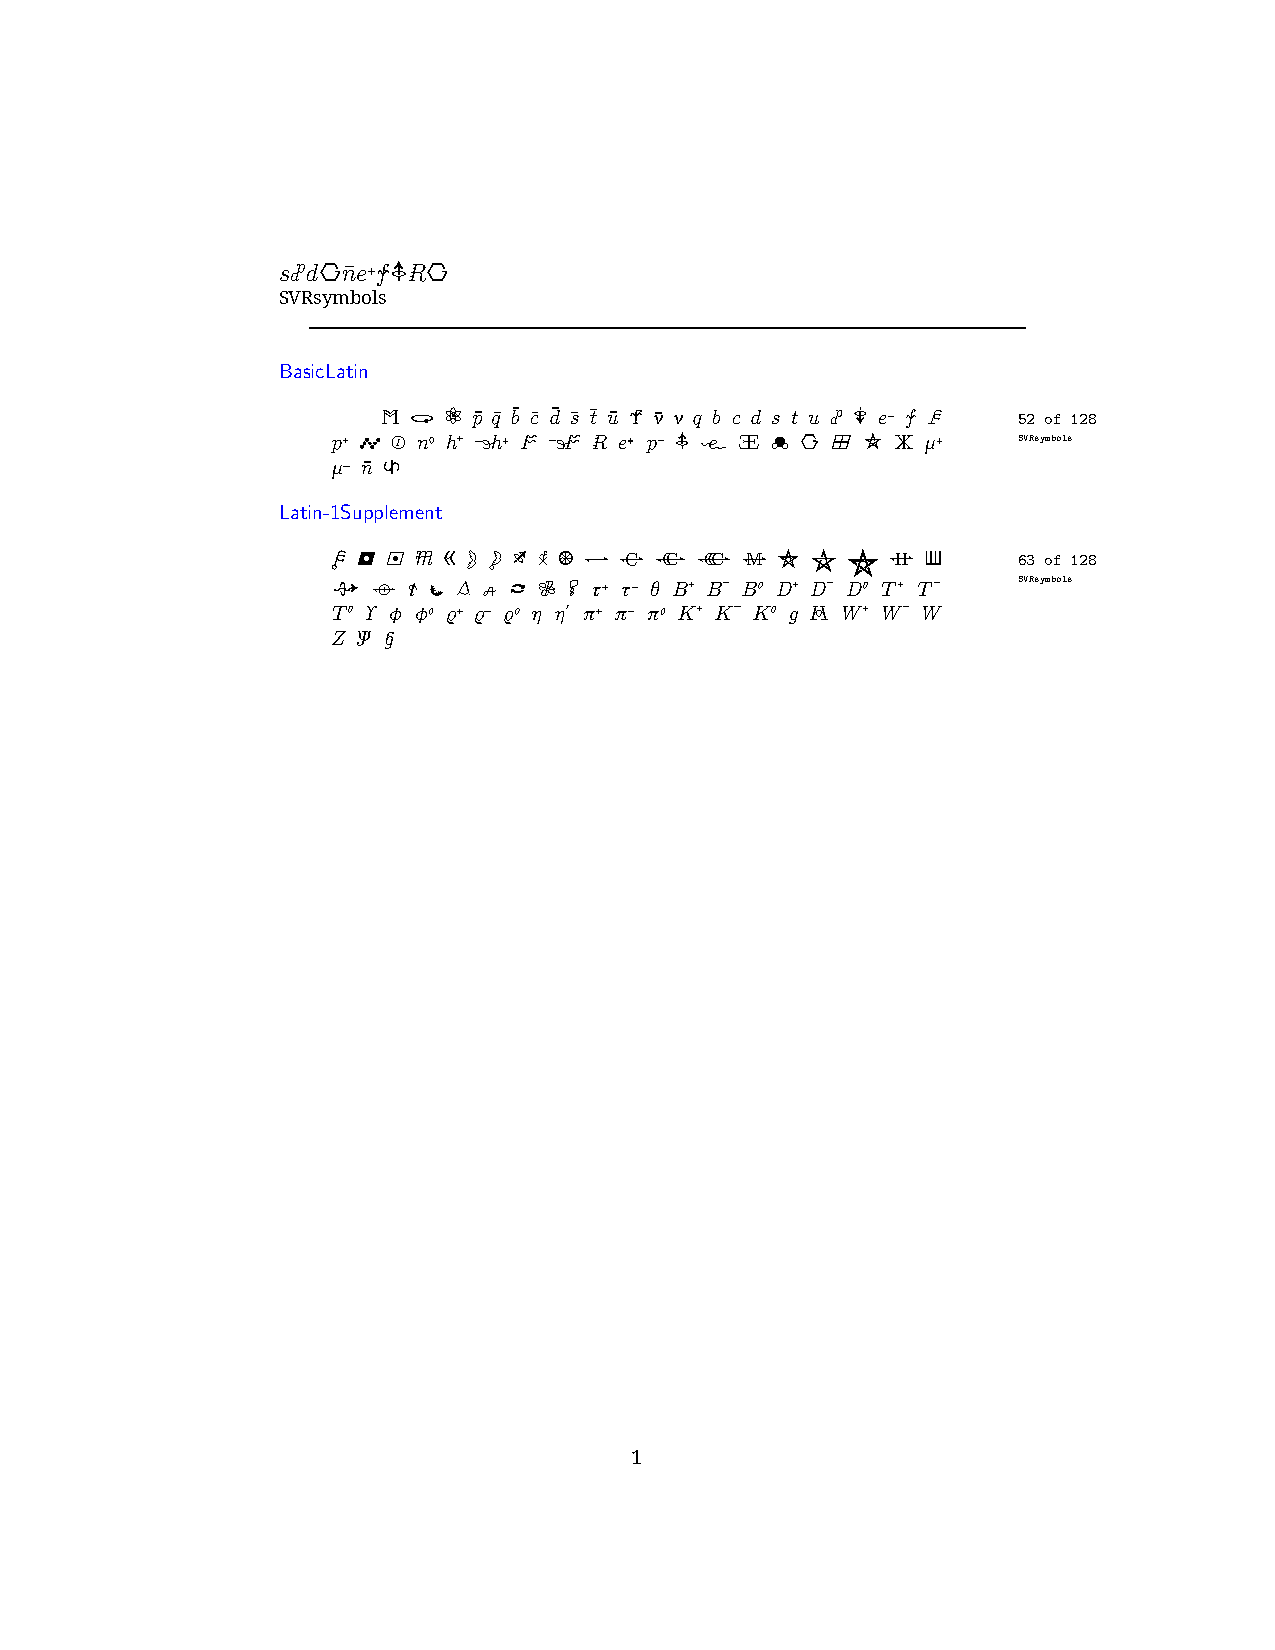
\includepdf[pages=1,nup=1x1,frame=true]{font-unicode-blocks-SVRsymbols}













\end{document}